
\documentclass[]{article}
\usepackage{amsmath}
\usepackage{graphics}
\usepackage{graphicx}
\begin{document}




\section*{Bias and Variance}

You train a learning algorithm, and find that it has unacceptably high error on the test set. You plot the learning curve, and obtain the figure below. 

Is the algorithm suffering from high bias, high variance, or neither?

\begin{figure}[h!]
\centering
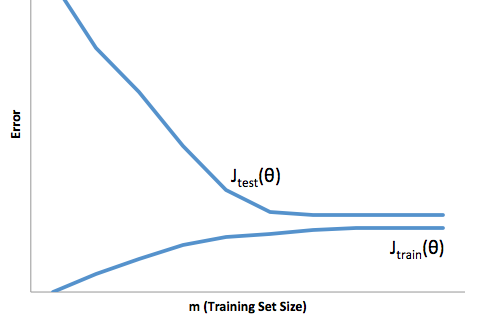
\includegraphics[width=0.7\linewidth]{C:/Users/Computer5/Dropbox/Public/ML-Coursera/MLQuiz10Q1}
\label{fig:MLQuiz10Q1}
\end{figure}

\begin{itemize}
\item[(i)] \textbf{Neither	}		

\item[(ii)] \textbf{High bias}			

\item[(iii)] \textbf{High variance}	This learning curve shows high error on both the training and test sets, so the algorithm is suffering from high bias.
\end{itemize}
\end{document}